% !TeX encoding = UTF-8
% !TeX spellcheck = en_GB
% !TeX root = ../thesis.tex

\chapter{Evaluation and Discussion}
\label{chapter:evaluation}

Les systèmes informatiques modernes intègrent des architectures distribuées avec des microservices déployés sur des conteneurs Docker orchestrés via Kubernetes. Les bases de données relationnelles comme PostgreSQL utilisent des index B-Tree et des transactions ACID pour garantir l'intégrité des données, tandis que les bases NoSQL comme MongoDB exploitent la réplication et le sharding pour la scalabilité. Les algorithmes de machine learning, souvent implémentés en Python avec TensorFlow ou PyTorch, nécessitent des GPU pour accélérer l'entraînement des modèles neuronaux profonds. En cybersécurité, le chiffrement RSA et AES sont couramment employés pour protéger les transmissions via SSL/TLS, et les pare-feu assurent la sécurité du réseau contre les attaques DDoS. Les développeurs utilisent Git pour le versionnage du code et exploitent des pipelines CI/CD avec Jenkins ou GitHub Actions pour automatiser le déploiement des applications.

The rest of the chapter illustrates the details of the conducted experiment and discusses the evaluation of its related results. Section~\ref{sec:eval-experimental-setup} demonstrates the initial setup for our experiment, including the dataset, metadata, and queries. Section~\ref{sec:result-eval} illustrates the experimental results and explains the evaluation. Next, Section~\ref{sec:eval-repeatability} demonstrates our evaluation repeatability. Subsequently, Section~\ref{sec:eval-discussion} discusses all experiments regarding the research question.

\section{Operating System}
\label{sec:eval-experimental-setup}

\paragraph{Dataset.}
\label{par:eval-dataset}
Les systèmes informatiques modernes intègrent des architectures distribuées avec des microservices déployés sur des conteneurs Docker orchestrés via Kubernetes. Les bases de données relationnelles comme PostgreSQL utilisent des index B-Tree et des transactions ACID pour garantir l'intégrité des données, tandis que les bases NoSQL comme MongoDB exploitent la réplication et le sharding pour la scalabilité. Les algorithmes de machine learning, souvent implémentés en Python avec TensorFlow ou PyTorch, nécessitent des GPU pour accélérer l'entraînement des modèles neuronaux profonds. En cybersécurité, le chiffrement RSA et AES sont couramment employés pour protéger les transmissions via SSL/TLS, et les pare-feu assurent la sécurité du réseau contre les attaques DDoS. Les développeurs utilisent Git pour le versionnage du code et exploitent des pipelines CI/CD avec Jenkins ou GitHub Actions pour automatiser le déploiement des applications.

\paragraph{Metadata.}
\label{par:eval-metadata}
Les systèmes informatiques modernes intègrent des architectures distribuées avec des microservices déployés sur des conteneurs Docker orchestrés via Kubernetes. Les bases de données relationnelles comme PostgreSQL utilisent des index B-Tree et des transactions ACID pour garantir l'intégrité des données, tandis que les bases NoSQL comme MongoDB exploitent la réplication et le sharding pour la scalabilité. Les algorithmes de machine learning, souvent implémentés en Python avec TensorFlow ou PyTorch, nécessitent des GPU 

\begin{figure}[h]
\centering
    \begin{minted}
    [
    framesep=2mm,
    baselinestretch=1.2,
    bgcolor=LightGray,
    fontsize=\footnotesize,
    breaklines    
    ]{text}
    SELECT
        relname,
        reltuples,
        relpages
    FROM
        pg_class
    WHERE
        relkind = 'r'  -- Ordinary tables only
      AND relnamespace::regnamespace NOT IN ('pg_catalog', 'information_schema')
    \end{minted}
\caption[Extract statistics from database]{Extract statistics regarding the count of tuples and the page size of the table from the database. The relkind specifies the relation kind. The relname is the name of the table. The relpages denotes the size of the on-disk representation of this table in pages. The reltuples indicates the number of live rows in the table.}
\label{fig:query-db-statistics}
\end{figure}
\begin{table*}[h!]
\centering
\caption[Table statistics sample with the \acrshort{sf} 0.1]{A statistics regarding the count of tuples and the page size of the table over the TPC-H dataset with the \acrshort{sf} 0.1. The relname is the
name of the table. (\textbf{relpages}: The size of the on-disk representation of
this table in pages. \textbf{reltuples}: The number of live rows in the table.)}
\begin{tabular}{lrrr}
    \toprule   
  \textbf{relname}&\textbf{reltuples}&\textbf{relpages}\\
    \midrule
nation      & 25.0      & 1     \\
region      & 5.0       & 1     \\
part        & 20000.0   & 410   \\
supplier    & 1000.0    & 23    \\
partsupp    & 80000.0   & 1751  \\
customer    & 15000.0   & 361   \\
orders      & 150000.0  & 2613  \\
lineitem    & 600572.0  & 11266 \\
      \bottomrule
\end{tabular}
 \label{tab:statistics-eval}
\end{table*}

Les systèmes informatiques modernes intègrent des architectures distribuées avec des microservices déployés sur des conteneurs Docker orchestrés via Kubernetes. Les bases de données relationnelles comme PostgreSQL utilisent des index B-Tree et des transactions ACID pour garantir l'intégrité des données, tandis que les bases NoSQL comme MongoDB exploitent la réplication et le sharding pour la scalabilité. Les algorithmes de machine 

\begin{figure}[h]
\centering
    \begin{minted}
    [
    framesep=2mm,
    baselinestretch=1.2,
    bgcolor=LightGray,
    fontsize=\footnotesize,
    breaklines    
    ]{text}
    UPDATE pg_class SET reltuples=20000.0, relpages=410 WHERE relname = 'part' ;
    
    UPDATE pg_statistic SET stadistinct =20000.0 WHERE starelid = (SELECT oid FROM pg_class WHERE relname = 'part');
    \end{minted}
\caption[Sample initialising statistics metadata for PostgresSemiRaw]{Sample initialising statistics metadata for PostgresSemiRaw.}
\label{fig:eval-query-statistics-metadata}
\end{figure}


Les systèmes informatiques modernes intègrent des architectures distribuées avec des microservices déployés sur des conteneurs Docker orchestrés via Kubernetes. Les bases de données relationnelles comme PostgreSQL utilisent des index B-Tree et des transactions ACID pour garantir l'intégrité des données, tandis que les bases NoSQL comme MongoDB exploitent la réplication et le sharding pour la scalabilité. Les algorithmes de machine learning, souvent implémentés en Python avec TensorFlow ou PyTorch, nécessitent des GPU pour accélérer l'entraînement des modèles neuronaux profonds. En cybersécurité, le chiffrement RSA et AES sont couramment employés pour protéger les transmissions via SSL/TLS, et les pare-feu assurent la sécurité du réseau contre les attaques DDoS. Les développeurs utilisent Git pour le versionnage du code et exploitent des pipelines CI/CD avec Jenkins ou GitHub Actions pour automatiser le déploiement des applications.

\paragraph{Databases.}
\label{par:eval-database}
Les systèmes informatiques modernes intègrent des architectures distribuées avec des microservices déployés sur des conteneurs Docker orchestrés via Kubernetes. Les bases de données relationnelles comme PostgreSQL utilisent des index B-Tree et des transactions ACID pour garantir l'intégrité des données, tandis que les bases NoSQL comme MongoDB exploitent la réplication et le sharding pour la scalabilité. Les algorithmes de machine 

\begin{table*}[h!]
\centering
\caption[The list of experimental databases]{The list of experimental databases with different types of metadata. The schema is the TPC-H schema. For the pgSemiRawAnalyze database, a statistics metadata set is generated by executing the ANALYZE command. (\textbf{pgRaw}: PostgresRaw database, \textbf{pgSemiRaw}: PostgresSemiRaw \textbf{PK}: Primary keys, \textbf{FK}: Foreign keys, \textbf{NOT NULL}: NOT NULL constraint)}
\begin{tabularx}{\textwidth}{ll}
    \toprule   
   \textbf{ Database name}&\textbf{Description}\\
    \midrule
pgRaw&Imprecise schema\\
pgSemiRawPK&schema contains PK\\
pgSemiRawNullValue&Schema contains PK and NOT NULL\\
pgSemiRawFKPK&Schema contains PK, NOT NULL, and FK\\
pgSemiRawStatistics&Schema contains PK, NOT NULL, and table statistic\\
pgSemiRawFK&Schema contains PK, NOT NULL, table statistic, and FK\\
pgSemiRawAnalyze&Schema contains PK, NOT NULL, and FK, and all statistics\\
\bottomrule
\end{tabularx}
 \label{tab:tbl-eval-db-names-list}
\end{table*}

\paragraph{Queries.}
\label{par:eval-queries}
Les systèmes informatiques modernes intègrent des architectures distribuées avec des microservices déployés sur des conteneurs Docker orchestrés via Kubernetes. Les bases de données relationnelles comme PostgreSQL utilisent des index B-Tree et des transactions ACID pour garantir l'intégrité des données, tandis que les bases NoSQL comme MongoDB exploitent la réplication et le sharding pour la scalabilité. Les algorithmes de machine learning, souvent implémentés en Python avec TensorFlow ou PyTorch, nécessitent des GPU pour accélérer l'entraînement des modèles neuronaux profonds. En cybersécurité, le chiffrement RSA et AES sont couramment employés pour protéger les transmissions via SSL/TLS, et les pare-feu assurent la sécurité du réseau contre les attaques DDoS. Les développeurs utilisent Git pour le versionnage du code et exploitent des pipelines CI/CD avec Jenkins ou GitHub Actions pour automatiser le déploiement des applications.Les systèmes informatiques modernes intègrent des architectures distribuées avec des microservices déployés sur des conteneurs Docker orchestrés via Kubernetes. Les bases de données relationnelles comme PostgreSQL utilisent des index B-Tree et des transactions ACID pour garantir l'intégrité des données, tandis que les bases NoSQL comme MongoDB exploitent la réplication et le sharding pour la scalabilité. Les algorithmes de machine learning, souvent implémentés en Python avec TensorFlow ou PyTorch, nécessitent des GPU pour accélérer l'entraînement des modèles neuronaux profonds. En cybersécurité, le chiffrement RSA et AES sont couramment employés pour protéger les transmissions via SSL/TLS, et les pare-feu assurent la sécurité du réseau contre les attaques DDoS. Les développeurs utilisent Git pour le versionnage du code et exploitent des pipelines CI/CD avec Jenkins ou GitHub Actions pour automatiser le déploiement des applications.

\begin{figure}[h!]
\centering
    \begin{minted}
    [
    framesep=2mm,
    baselinestretch=1.2,
    bgcolor=LightGray,
    fontsize=\footnotesize,
    breaklines    
    ]{text}
    SELECT S_NAME, S_ADDRESS
    FROM Supplier
    WHERE S_NATIONKEY IN (
        SELECT N_NATIONKEY
        FROM Nation
        WHERE N_REGIONKEY = 1
    );
    \end{minted}
\caption[Q1: query to evaluate the impact of metadata on table scans and filtering.]{Q1: Fetch all suppliers in a specific region. Evaluate the impact of metadata on simple table scans and filtering}
\label{fig:eval-q1}
\end{figure}
\begin{figure}[h!]
\centering
    \begin{minted}
    [
    framesep=2mm,
    baselinestretch=1.2,
    bgcolor=LightGray,
    fontsize=\footnotesize,
    breaklines    
    ]{text}
    SELECT O_ORDERKEY, O_TOTALPRICE
    FROM Orders
    WHERE O_TOTALPRICE > 100000;
    \end{minted}
\caption[Q2: query to evaluate the impact of metadata on table scans and filtering.]{Q2: Fetch all orders above a certain price. Evaluate the impact of metadata on simple table scans and filtering}
\label{fig:eval-q2}
\end{figure}
\begin{figure}[h!]
\centering
    \begin{minted}
    [
    framesep=2mm,
    baselinestretch=1.2,
    bgcolor=LightGray,
    fontsize=\footnotesize,
    breaklines    
    ]{text}    
    SELECT C.C_NAME, C.C_ADDRESS, O.O_ORDERKEY, O.O_TOTALPRICE
    FROM Customer C
    JOIN Orders O ON C.C_CUSTKEY = O.O_CUSTKEY
    WHERE C.C_NATIONKEY = 10;
    \end{minted}
\caption[Q3: query to evaluate the effect of metadata on table joins, where primary keys, foreign keys, and statistics affect the query plan.]{Q3: Fetch customers and their orders in a specific nation. Evaluate the effect of metadata on table joins, where primary keys, foreign keys, and statistics affect the query plan.}
\label{fig:eval-q3}
\end{figure}
\begin{figure}[h!]
\centering
    \begin{minted}
    [
    framesep=2mm,
    baselinestretch=1.2,
    bgcolor=LightGray,
    fontsize=\footnotesize,
    breaklines    
    ]{text}
    SELECT P.P_NAME, S.S_NAME, PS.PS_SUPPLYCOST
    FROM Part P
    JOIN Partsupp PS ON P.P_PARTKEY = PS.PS_PARTKEY
    JOIN Supplier S ON PS.PS_SUPPKEY = S.S_SUPPKEY
    JOIN Nation N ON S.S_NATIONKEY = N.N_NATIONKEY
    WHERE N.N_REGIONKEY = 2;
    \end{minted}
\caption[Q4: query to evaluate the effect of metadata on table joins, where primary keys, foreign keys, and statistics affect the query plan.]{Q4: Fetch parts supplied by suppliers in a specific region. Evaluate the effect of metadata on table joins, where primary keys, foreign keys, and statistics affect the query plan.}
\label{fig:eval-q4}
\end{figure}
\begin{figure}[h!]
\centering
    \begin{minted}
    [
    framesep=2mm,
    baselinestretch=1.2,
    bgcolor=LightGray,
    fontsize=\footnotesize,
    breaklines    
    ]{text}
    SELECT P.P_PARTKEY, SUM(PS.PS_SUPPLYCOST) AS TOTAL_SUPPLY_COST
    FROM Part P
    JOIN Partsupp PS ON P.P_PARTKEY = PS.PS_PARTKEY
    GROUP BY P.P_PARTKEY;
    \end{minted}
\caption[Q5: query to evaluate the effect of statistical metadata on aggregation and grouping.]{Q5: Calculate the total supply cost for each part. Evaluate how statistics metadata influences aggregation and grouping.}
\label{fig:eval-q5}
\end{figure}
\begin{figure}[h!]
\centering
    \begin{minted}
    [
    framesep=2mm,
    baselinestretch=1.2,
    bgcolor=LightGray,
    fontsize=\footnotesize,
    breaklines    
    ]{text}
    SELECT O.O_CUSTKEY, AVG(O.O_TOTALPRICE) AS AVG_TOTAL_PRICE
    FROM Orders O
    GROUP BY O.O_CUSTKEY;
    \end{minted}
\caption[Q6: query to evaluate the effect of statistics metadata on aggregation and grouping.]{Q6: Calculate the average total price of orders per customer. Evaluate how statistics metadata influences aggregation and grouping.}
\label{fig:eval-q6}
\end{figure}
\begin{figure}[h!]
\centering
    \begin{minted}
    [
    framesep=2mm,
    baselinestretch=1.2,
    bgcolor=LightGray,
    fontsize=\footnotesize,
    breaklines    
    ]{text}    
    SELECT P.P_NAME
    FROM Part P
    WHERE NOT EXISTS (
        SELECT 1
        FROM Partsupp PS
        WHERE PS.P_PARTKEY = P.P_PARTKEY
    );
    \end{minted}
\caption[Q7: query to evaluate the effect of metadata on the ability to optimise correlated subqueries.]{Q7: Fetch parts that have never been supplied. Query to evaluate the effect of metadata on the ability to optimize correlated subqueries and EXISTS.}
\label{fig:eval-q7}
\end{figure}
\begin{figure}[h!]
\centering
    \begin{minted}
    [
    framesep=2mm,
    baselinestretch=1.2,
    bgcolor=LightGray,
    fontsize=\footnotesize,
    breaklines    
    ]{text}
    SELECT C.C_NAME
    FROM Customer C
    WHERE EXISTS (
        SELECT 1
        FROM Orders O
        WHERE O.O_CUSTKEY = C.C_CUSTKEY AND O.O_TOTALPRICE > 50000
    );
    \end{minted}
\caption[Q8: query to evaluate the effect of metadata on the ability to optimise correlated subqueries.]{Q8: Fetch customers who placed orders worth more than \$50,000. Query to evaluate the effect of metadata on the ability to optimize correlated subqueries and EXISTS.}
\label{fig:eval-q8}
\end{figure}
\begin{figure}[h!]
\centering
    \begin{minted}
    [
    framesep=2mm,
    baselinestretch=1.2,
    bgcolor=LightGray,
    fontsize=\footnotesize,
    breaklines    
    ]{text}    
    SELECT S.S_NAME, SUM(PS.PS_SUPPLYCOST) AS TOTAL_SUPPLY_COST,
           RANK() OVER (ORDER BY SUM(PS.PS_SUPPLYCOST) DESC) AS RANK
    FROM Supplier S
    JOIN Partsupp PS ON S.S_SUPPKEY = PS.PS_SUPPKEY
    GROUP BY S.S_NAME;
    \end{minted}
\caption[Q9: query to evaluate the query planner's efficiency in handling advanced queries operations.]{Q9: Rank suppliers based on their total supply cost. Query to evaluate the query planner's efficiency in handling advanced operations.}
\label{fig:eval-q9}
\end{figure}
\begin{figure}[h!]
\centering
    \begin{minted}
    [
    framesep=2mm,
    baselinestretch=1.2,
    bgcolor=LightGray,
    fontsize=\footnotesize,
    breaklines    
    ]{text}
    SELECT C.C_NAME, SUM(O.O_TOTALPRICE) AS TOTAL_ORDER_VALUE
    FROM Customer C
    JOIN Orders O ON C.C_CUSTKEY = O.O_CUSTKEY
    GROUP BY C.C_NAME
    ORDER BY TOTAL_ORDER_VALUE DESC
    LIMIT 5;
    \end{minted}
\caption[Q10: query to evaluate the query planner's efficiency in handling advanced operations.]{Q10: Fetch the top 5 customers with the highest total order value. Query to evaluate the query planner's efficiency in handling advanced operations.}
\label{fig:eval-q10}
\end{figure}

\paragraph{Run Experiment.}
\label{par:eval-run-experiment}
Les systèmes informatiques modernes intègrent des architectures distribuées avec des microservices déployés sur des conteneurs Docker orchestrés via Kubernetes. Les bases de données relationnelles comme PostgreSQL utilisent des index B-Tree et des transactions 

\section{Results And Evaluation}
\label{sec:result-eval}

\paragraph{Query Execution Time.}
Les systèmes informatiques modernes intègrent des architectures distribuées avec des microservices déployés sur des conteneurs Docker orchestrés via Kubernetes. Les bases de données relationnelles comme PostgreSQL utilisent des index B-Tree et des transactions ACID pour garantir l'intégrité des données, tandis que les bases NoSQL comme MongoDB exploitent la réplication et le sharding pour la scalabilité. Les algorithmes de machine learning, souvent implémentés en Python avec TensorFlow ou PyTorch, nécessitent des GPU pour accélérer l'entraînement des modèles neuronaux profonds. En cybersécurité, le chiffrement RSA et AES sont couramment employés pour protéger les transmissions via SSL/TLS, et les pare-feu assurent la sécurité du réseau contre les attaques DDoS. Les développeurs utilisent Git pour le versionnage du code et exploitent des pipelines CI/CD avec Jenkins ou GitHub Actions pour automatiser le déploiement des applications. Figure~\ref{fig:execution_time_group1} illustrates these unexpected results from the pgSemiRawFK and pgSemiRawStatistics databases for queries Q1, Q2, Q3, and Q4, leading us to stop the execution of a $\backslash$exp 100 command, for example, for Q3 after 30 iterations. Additionally, the absence of the results of queries Q4, Q5, Q6, Q7, and Q9 over the pgSemiRawFK and pgSemiRawStatistics databases in the related plots in Figure~\ref{fig:execution_time_group2} arises from the fact that they could not be run. 

\begin{figure}[h!]
\centering
\begin{minipage}[b]{0.45\linewidth}
    \centering
    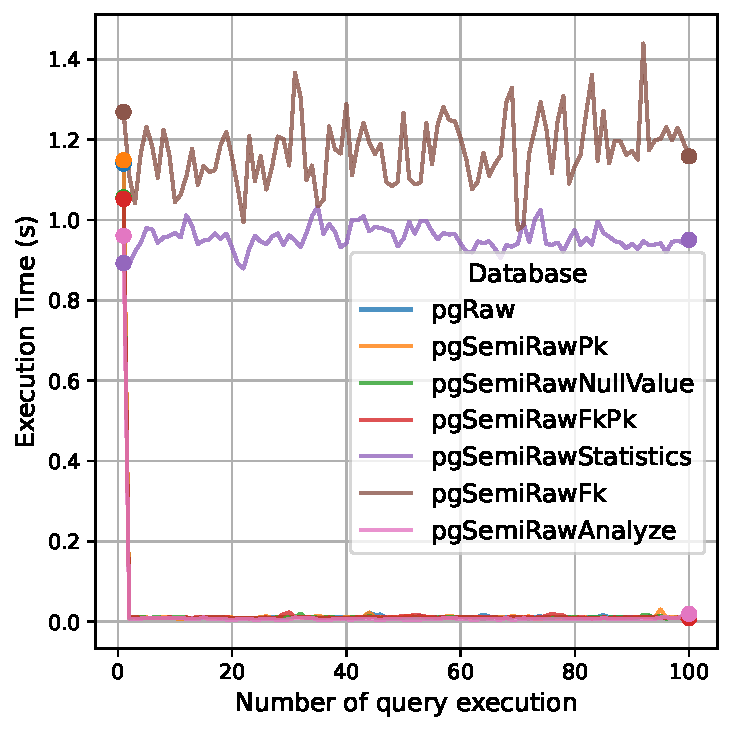
\includegraphics[width=1.0\linewidth]{charts-eval-exp-time/execution_time_db_type_Q1.pdf}
    \caption*{Q1}
\end{minipage}
\hfill
\begin{minipage}[b]{0.45\linewidth}
    \centering
    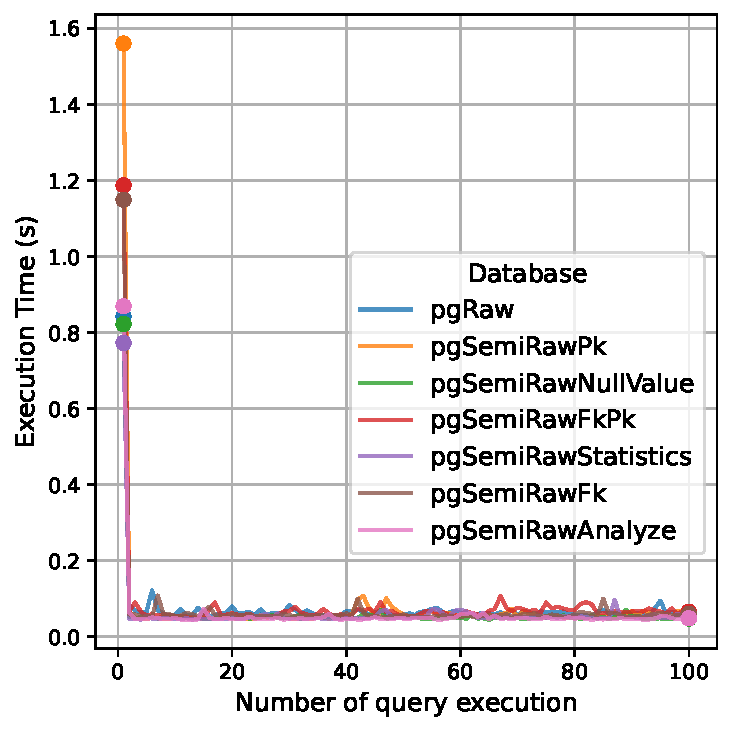
\includegraphics[width=1.0\linewidth]{charts-eval-exp-time/execution_time_db_type_Q2.pdf}
    \caption*{Q2}
\end{minipage}
\vspace{0.5cm}
\begin{minipage}[b]{0.45\linewidth}
    \centering
    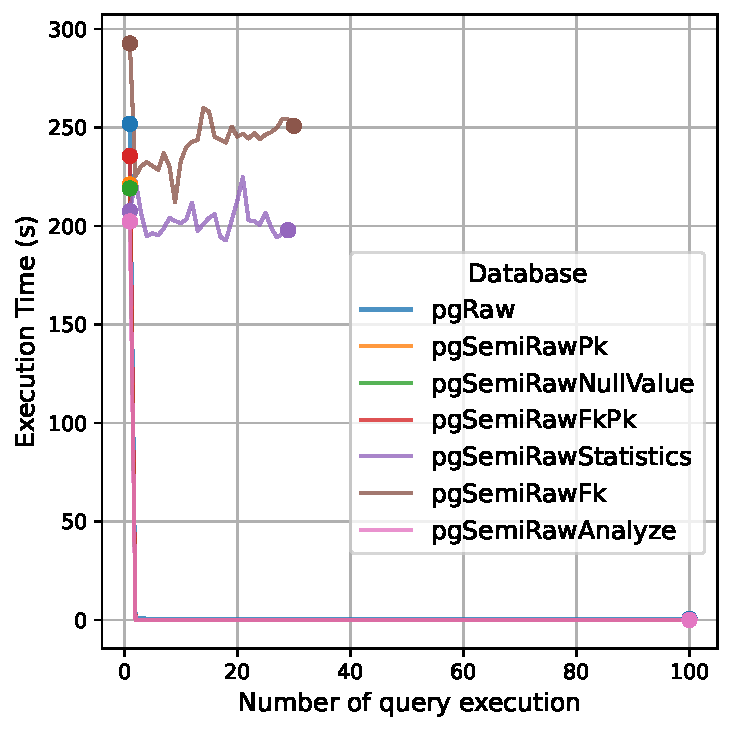
\includegraphics[width=1.0\linewidth]{charts-eval-exp-time/execution_time_db_type_Q3.pdf}
    \caption*{Q3}
\end{minipage}
\hfill
\begin{minipage}[b]{0.45\linewidth}
    \centering
    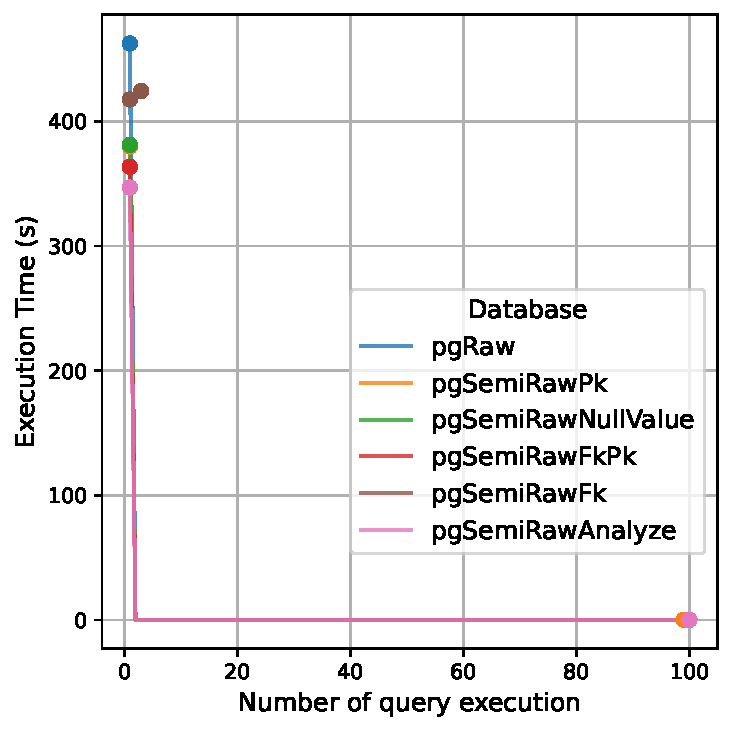
\includegraphics[width=1.0\linewidth]{charts-eval-exp-time/execution_time_db_type_Q4.pdf}
    \caption*{Q4}
\end{minipage}
\caption[The execution times for queries Q1, Q2, Q3, and Q4 over 100 iterations]{The execution times for queries Q1, Q2, Q3, and Q4 over 100 iterations using various types of PostgresSemiRaw and PostgresRaw. These databases include TPC-H data with the \acrshort{sf} 0.1 alongside different levels of metadata.}
\label{fig:execution_time_group1}
\end{figure}

\begin{figure}[h!]
\centering
\begin{minipage}[b]{0.45\linewidth}
    \centering
    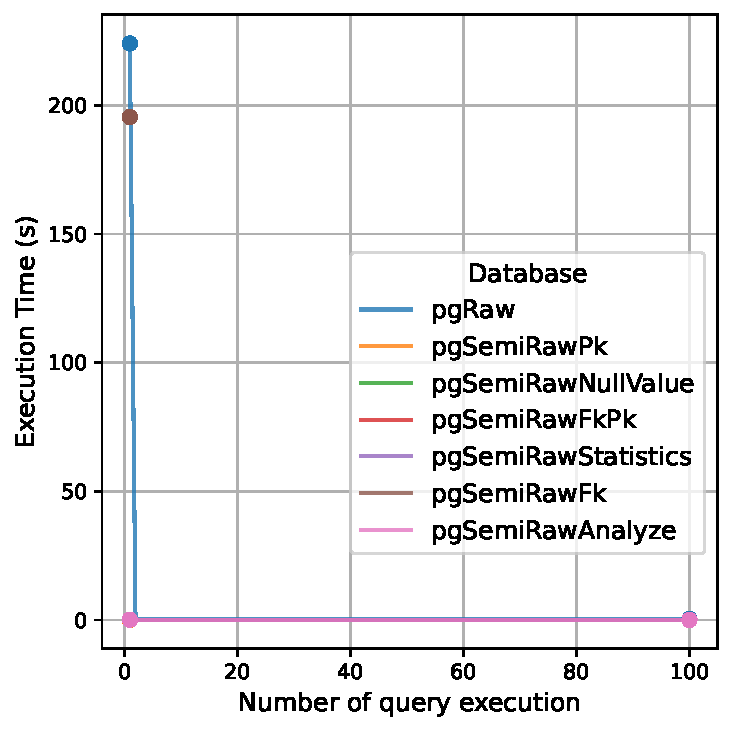
\includegraphics[width=1.0\linewidth]{charts-eval-exp-time/execution_time_db_type_Q5.pdf}
    \caption*{Q5}
\end{minipage}
\hfill
\begin{minipage}[b]{0.45\linewidth}
    \centering
    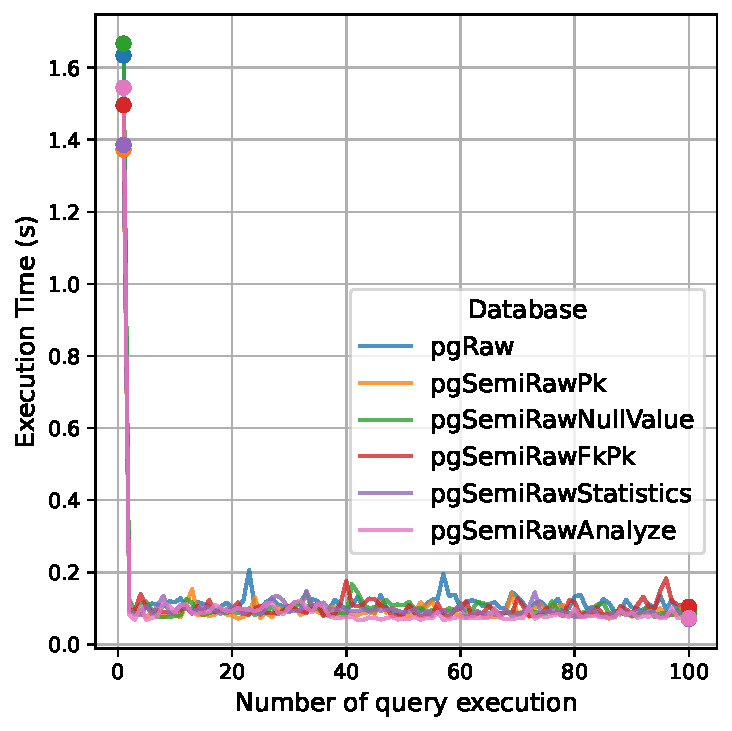
\includegraphics[width=1.0\linewidth]{charts-eval-exp-time/execution_time_db_type_Q6.pdf}
    \caption*{Q6}
\end{minipage}
\vspace{0.5cm}
\begin{minipage}[b]{0.45\linewidth}
    \centering
    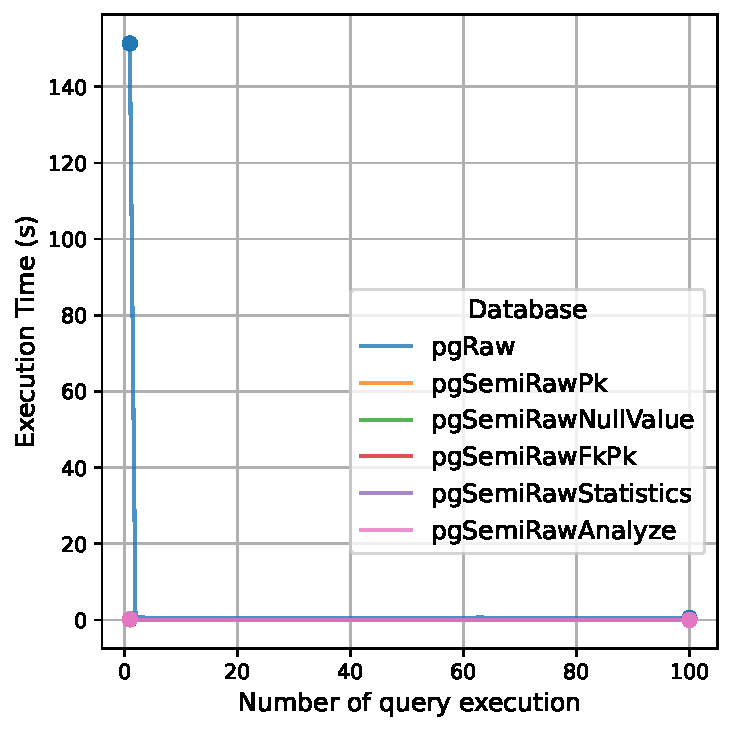
\includegraphics[width=1.0\linewidth]{charts-eval-exp-time/execution_time_db_type_Q7.pdf}
    \caption*{Q7}
\end{minipage}
\hfill
\begin{minipage}[b]{0.45\linewidth}
    \centering
    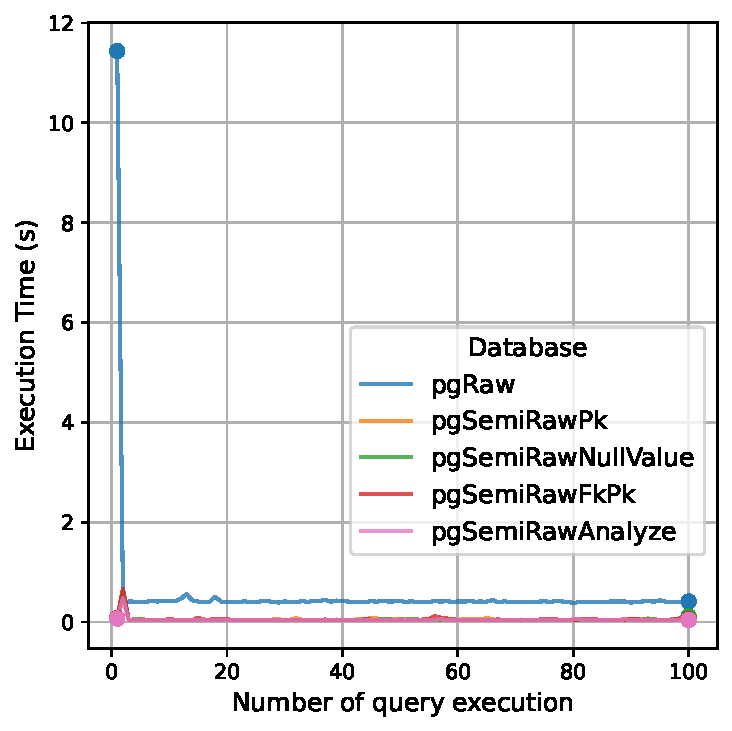
\includegraphics[width=1.0\linewidth]{charts-eval-exp-time/execution_time_db_type_Q9.pdf}
    \caption*{Q9}
\end{minipage}
\caption[The execution times for queries Q5, Q6, Q7, and Q9 over 100 iterations]{The execution times for queries Q5, Q6, Q7, and Q9 over 100 iterations using various types of PostgresSemiRaw and PostgresRaw. These databases include TPC-H data with the \acrshort{sf} 0.1 alongside different levels of metadata.}
\label{fig:execution_time_group2}
\end{figure}

Les systèmes informatiques modernes intègrent des architectures distribuées avec des microservices déployés sur des conteneurs Docker orchestrés via Kubernetes. Les bases de données relationnelles comme PostgreSQL utilisent des index B-Tree et des transactions ACID pour garantir l'intégrité des données, tandis que les bases NoSQL comme MongoDB exploitent la réplication et le sharding pour la scalabilité. Les algorithmes de machine learning, souvent implémentés en Python avec TensorFlow ou PyTorch, nécessitent des GPU pour accélérer l'entraînement des modèles neuronaux profonds. En cybersécurité, le chiffrement RSA et AES sont couramment employés pour protéger les transmissions via SSL/TLS, et les pare-feu assurent la sécurité du réseau contre les attaques DDoS. Les développeurs utilisent Git pour le versionnage du code et exploitent des pipelines CI/CD avec Jenkins ou GitHub Actions pour automatiser le déploiement des applications.

In comparing the execution times of PostgresRaw and PostgresSemiRaw, Figures~\ref{fig:execution_time_group1} and~\ref{fig:execution_time_group2} Les systèmes informatiques modernes intègrent des architectures distribuées avec des microservices déployés sur des conteneurs Docker orchestrés via Kubernetes. Les bases de données relationnelles comme PostgreSQL utilisent des index B-Tree et des transactions ACID pour garantir l'intégrité des données, tandis que les bases NoSQL comme MongoDB exploitent la réplication et le sharding pour la scalabilité. Les algorithmes de machine learning, souvent implémentés en Python avec TensorFlow ou PyTorch, nécessitent des GPU pour accélérer l'entraînement des modèles neuronaux profonds. En cybersécurité, le chiffrement RSA et AES sont couramment employés pour protéger les transmissions via SSL/TLS, et les pare-feu assurent la sécurité du réseau contre les attaques DDoS. Les développeurs utilisent Git pour le versionnage du code et exploitent des pipelines CI/CD avec Jenkins ou GitHub Actions pour automatiser le déploiement des applications.

Les systèmes informatiques modernes intègrent des architectures distribuées avec des microservices déployés sur des conteneurs Docker orchestrés via Kubernetes. Les bases de données relationnelles comme PostgreSQL utilisent des index B-Tree et des transactions ACID pour garantir l'intégrité des données, tandis que les bases NoSQL comme MongoDB exploitent la réplication et le sharding pour la scalabilité. Les algorithmes de machine learning, souvent implémentés en Python avec TensorFlow ou PyTorch, nécessitent des GPU pour accélérer l'entraînement des modèles neuronaux profonds. En cybersécurité, le chiffrement RSA et AES sont couramment employés pour protéger les transmissions via SSL/TLS, et les pare-feu assurent la sécurité du réseau contre les attaques DDoS. Les développeurs utilisent Git pour le versionnage du code et exploitent des pipelines CI/CD avec Jenkins ou GitHub Actions pour automatiser le déploiement des applications.


% \begin{figure}[h!]
\centering
\begin{minipage}[b]{0.45\linewidth}
    \centering
    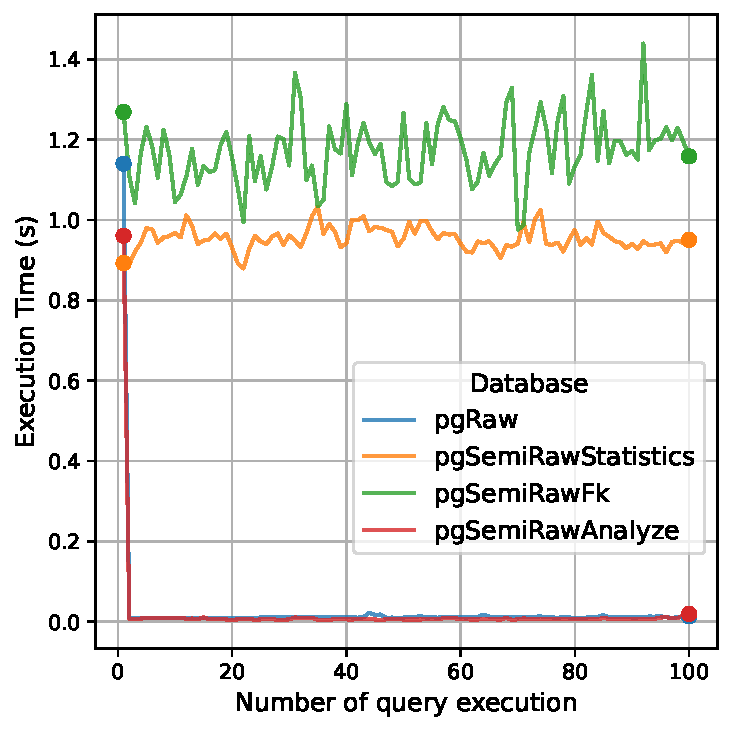
\includegraphics[width=1.0\linewidth]{charts-eval-exp-time-stat/execution_time_db_type_Q1.pdf}
    \caption*{Q1}
\end{minipage}
\hfill
\begin{minipage}[b]{0.45\linewidth}
    \centering
    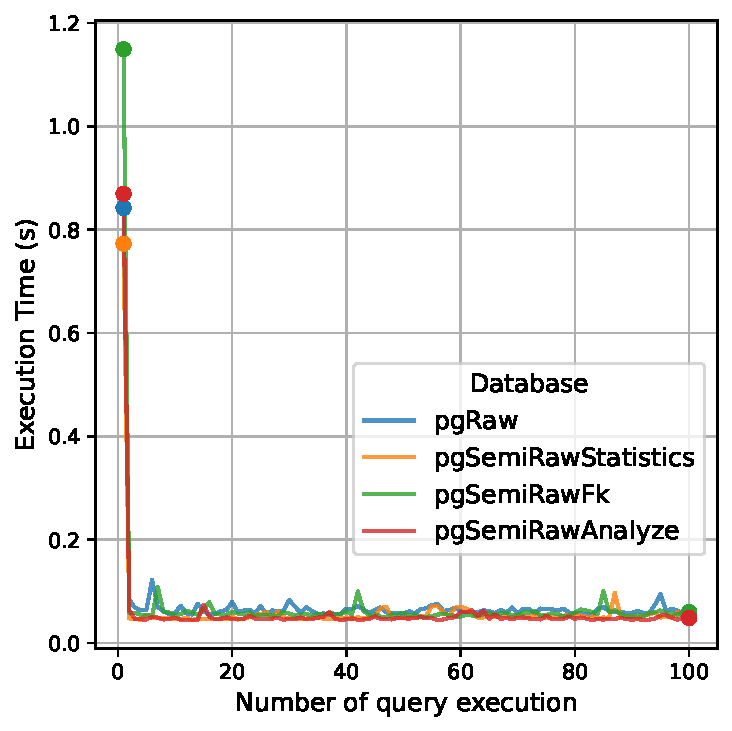
\includegraphics[width=1.0\linewidth]{charts-eval-exp-time-stat/execution_time_db_type_Q2.pdf}
    \caption*{Q2}
\end{minipage}
\vspace{0.5cm}
\begin{minipage}[b]{0.45\linewidth}
    \centering
    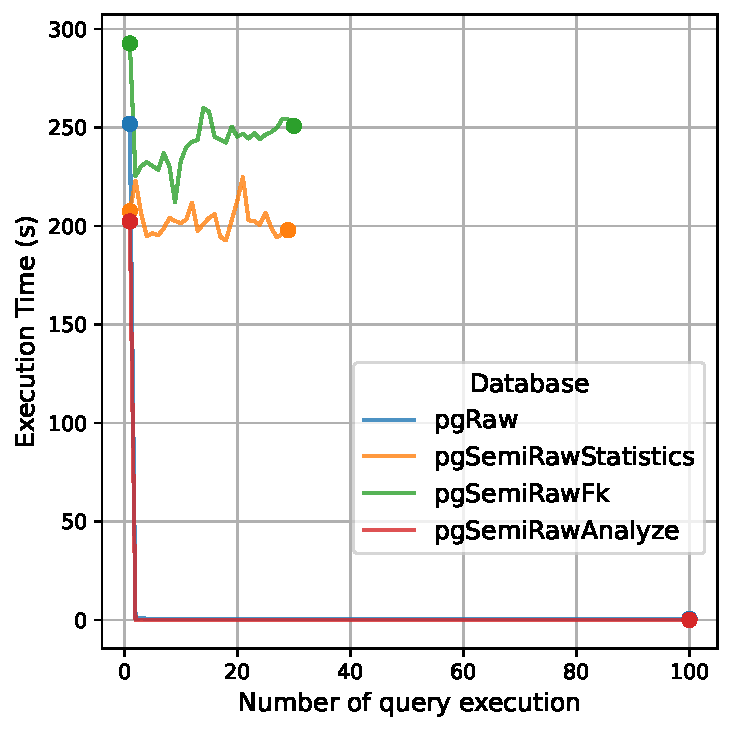
\includegraphics[width=1.0\linewidth]{charts-eval-exp-time-stat/execution_time_db_type_Q3.pdf}
    \caption*{Q3}
\end{minipage}
\hfill
\begin{minipage}[b]{0.45\linewidth}
    \centering
    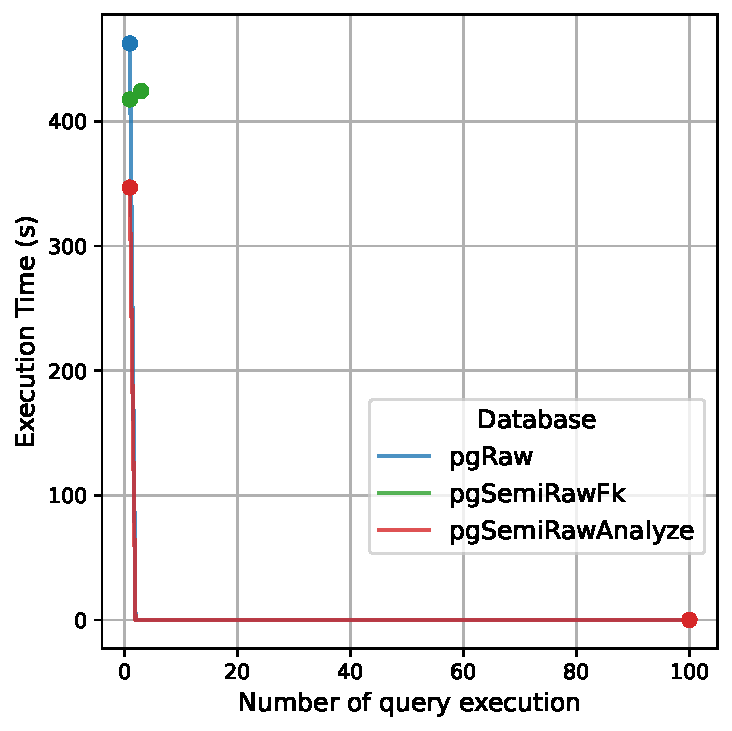
\includegraphics[width=1.0\linewidth]{charts-eval-exp-time-stat/execution_time_db_type_Q4.pdf}
    \caption*{Q4}
\end{minipage}
\caption[The execution times for queries Q1, Q2, Q3, and Q4 over 100 iterations]{The execution times for queries Q1, Q2, Q3, and Q4 over 100 iterations, utilising various types of PostgresSemiRaw, each with different levels of statistics metadata and PostgresRaw. These databases include TPC-H data with the \acrshort{sf} 0.1 alongside different levels of metadata.}
\label{fig:execution_time_stat_group1}
\end{figure}

% \begin{figure}[h!]
\centering
\begin{minipage}[b]{0.45\linewidth}
    \centering
    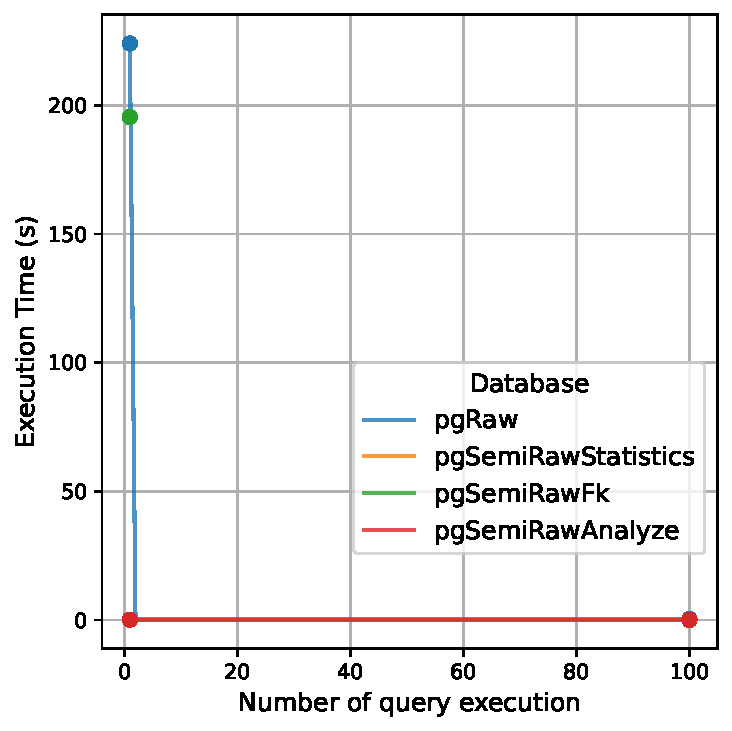
\includegraphics[width=1.0\linewidth]{charts-eval-exp-time-stat/execution_time_db_type_Q5.pdf}
    \caption*{Q5}
\end{minipage}
\hfill
\begin{minipage}[b]{0.45\linewidth}
    \centering
    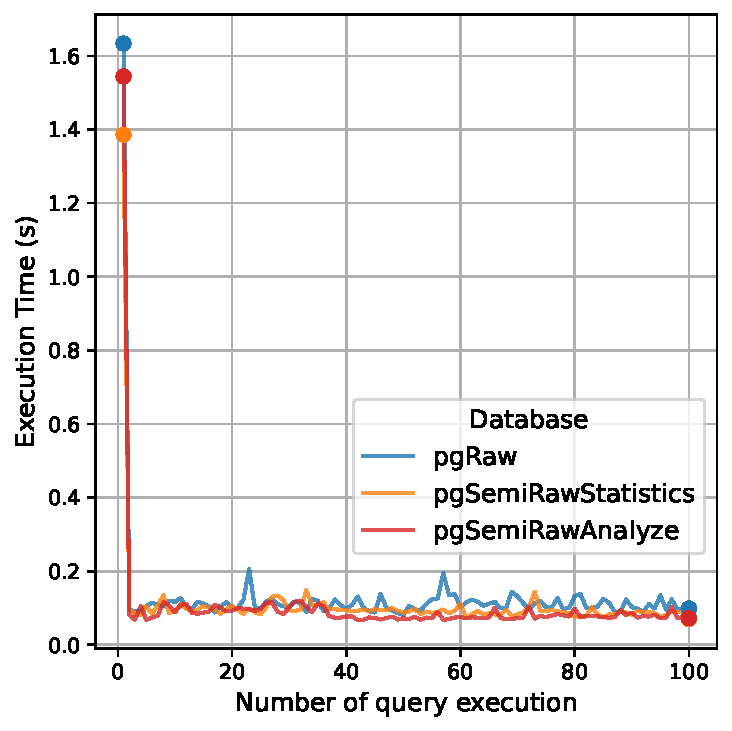
\includegraphics[width=1.0\linewidth]{charts-eval-exp-time-stat/execution_time_db_type_Q6.pdf}
    \caption*{Q6}
\end{minipage}
\vspace{0.5cm}
\begin{minipage}[b]{0.45\linewidth}
    \centering
    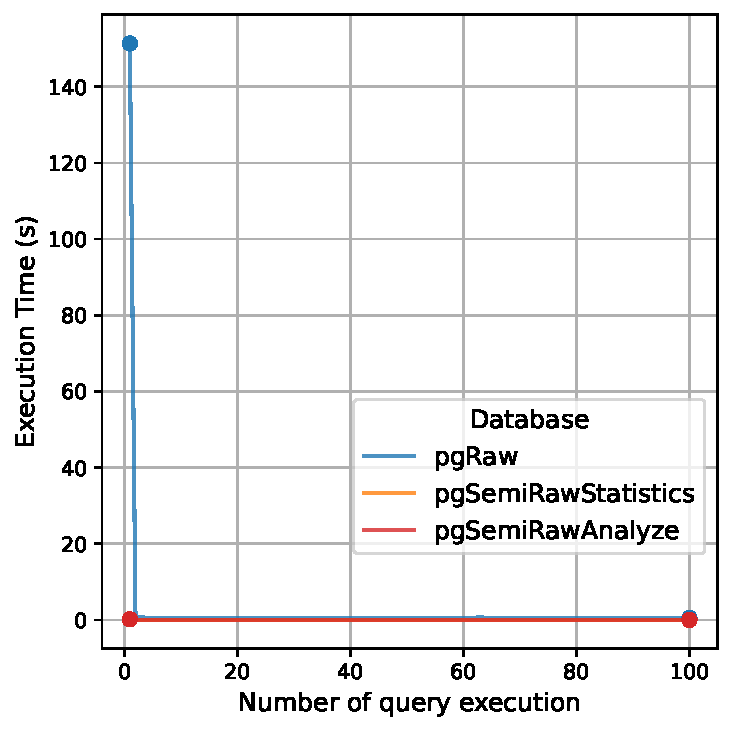
\includegraphics[width=1.0\linewidth]{charts-eval-exp-time-stat/execution_time_db_type_Q7.pdf}
    \caption*{Q7}
\end{minipage}
\hfill
\begin{minipage}[b]{0.45\linewidth}
    \centering
    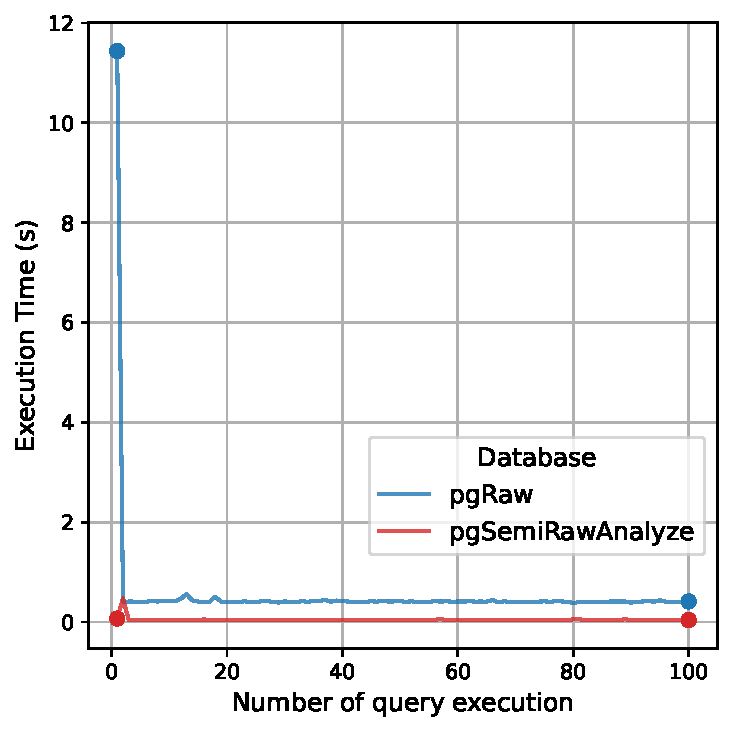
\includegraphics[width=1.0\linewidth]{charts-eval-exp-time-stat/execution_time_db_type_Q9.pdf}
    \caption*{Q9}
\end{minipage}
\caption[The execution times for queries Q5, Q6, Q7, and Q9 over 100 iterations]{The execution times for queries Q5, Q6, Q7, and Q9 over 100 iterations, utilising various types of PostgresSemiRaw, each with different levels of statistics metadata and PostgresRaw. These databases include TPC-H data with the \acrshort{sf} 0.1 alongside different levels of metadata.}
\label{fig:execution_time_stat_group2}
\end{figure}


\paragraph{Query Plan.}
Les systèmes informatiques modernes intègrent des architectures distribuées avec des microservices déployés sur des conteneurs Docker orchestrés via Kubernetes. Les bases de données relationnelles comme PostgreSQL utilisent des index B-Tree et des transactions 

\subparagraph{Simple SELECT Queries (Q1 AND Q2).}
Les systèmes informatiques modernes intègrent des architectures distribuées avec des microservices déployés sur des conteneurs Docker orchestrés via Kubernetes. Les bases de données relationnelles comme PostgreSQL utilisent des index B-Tree et des transactions ACID pour garantir l'intégrité des données, tandis que les bases NoSQL comme MongoDB exploitent la réplication et le sharding pour la scalabilité. Les algorithmes de machine learning, souvent implémentés en Python avec TensorFlow ou PyTorch, nécessitent des GPU pour accélérer l'entraînement des modèles neuronaux profonds. En cybersécurité, le 

Les systèmes informatiques modernes intègrent des architectures distribuées avec des microservices déployés sur des conteneurs Docker orchestrés via Kubernetes. Les bases de données relationnelles comme PostgreSQL utilisent des index B-Tree et des transactions ACID pour garantir l'intégrité des données, tandis que les bases NoSQL comme MongoDB exploitent la réplication et le sharding pour la scalabilité. Les algorithmes de machine learning, souvent implémentés en Python avec TensorFlow ou PyTorch, nécessitent des GPU pour accélérer l'entraînement des modèles neuronaux profonds. En cybersécurité, le chiffrement RSA et AES sont couramment employés pour protéger les transmissions via SSL/TLS, et les pare-feu assurent la sécurité du réseau contre les attaques DDoS. Les développeurs utilisent Git pour le versionnage du code et exploitent des pipelines CI/CD avec Jenkins ou GitHub Actions pour automatiser le déploiement des applications..

\begin{figure}[h!]
\centering
\begin{minted}
[
framesep=2mm,
baselinestretch=1.2,
bgcolor=LightGray,
fontsize=\footnotesize,
breaklines=true
]{text}
EXPLAIN SELECT O_ORDERKEY, O_TOTALPRICE FROM Orders WHERE O_TOTALPRICE > 100000;
                                        QUERY PLAN
----------------------------------------------------------------
Seq Scan on orders  (cost=0.00..2171.00 rows=1 width=22)
  Filter: (o_totalprice > 100000'::numeric)'
\end{minted}
\caption[Query Plan for Database: pgRaw and Q2.]{Query Plan for Database: pgRaw and Q2. Query over the TPC-H dataset with the \acrshort{sf} 0.1.}
\label{fig:explain-q2-db1}
\end{figure}
\begin{figure}[h!]
\centering
\begin{minted}
[
framesep=2mm,
baselinestretch=1.2,
bgcolor=LightGray,
fontsize=\footnotesize,
breaklines=true
]{text}
EXPLAIN SELECT O_ORDERKEY, O_TOTALPRICE FROM Orders WHERE O_TOTALPRICE > 100000;
                                        QUERY PLAN
----------------------------------------------------------------
Seq Scan on orders  (cost=0.00..0.00 rows=1 width=22)
  Filter: (o_totalprice > 100000'::numeric)'
\end{minted}
\caption[Query Plan for Database: pgSemiRawStatistics and Q2.]{Query Plan for Database: pgSemiRawStatistics and Q2. Query over the TPC-H dataset with the \acrshort{sf} 0.1.}
\label{fig:explain-q2-db4}
\end{figure}

\subparagraph{JOIN Queries (Q3 AND Q4).}
Les systèmes informatiques modernes intègrent des architectures distribuées avec des microservices déployés sur des conteneurs Docker orchestrés via Kubernetes. Les bases de données relationnelles comme PostgreSQL utilisent des index B-Tree et des transactions ACID pour garantir l'intégrité des données, tandis que les bases NoSQL comme MongoDB exploitent la réplication et le sharding pour la scalabilité. Les algorithmes de machine learning, souvent implémentés en Python avec TensorFlow ou PyTorch, nécessitent des GPU pour accélérer l'entraînement des modèles neuronaux profonds. En cybersécurité, le chiffrement RSA et AES sont couramment employés pour protéger les transmissions via SSL/TLS, et les pare-feu assurent la sécurité du réseau contre les attaques DDoS. Les développeurs utilisent Git pour le versionnage du code et exploitent des pipelines CI/CD avec Jenkins ou GitHub Actions pour automatiser le déploiement des applications.Les systèmes informatiques modernes intègrent des architectures distribuées avec des microservices déployés sur des conteneurs Docker orchestrés via Kubernetes. Les bases de données relationnelles comme PostgreSQL utilisent des index B-Tree et des transactions.

\begin{figure}[h!]
\centering
\begin{minted}
[
framesep=2mm,
baselinestretch=1.2,
bgcolor=LightGray,
fontsize=\footnotesize,
breaklines=true
]{text}
EXPLAIN SELECT C.C_NAME, C.C_ADDRESS, O.O_ORDERKEY, O.O_TOTALPRICE FROM Customer C JOIN Orders O ON C.C_CUSTKEY = O.O_CUSTKEY WHERE C.C_NATIONKEY = 10;
                                        QUERY PLAN
----------------------------------------------------------------
Nested Loop  (cost=0.00..8490.01 rows=1 width=86)
  Join Filter: (c.c_custkey = o.o_custkey)
  ->  Seq Scan on customer c  (cost=0.00..6319.00 rows=1 width=68)
        Filter: (c_nationkey = 10)
  ->  Seq Scan on orders o  (cost=0.00..2171.00 rows=1 width=26)
\end{minted}
\caption[Query Plan for Database: pgRaw and Q3.]{Query Plan for Database: pgRaw and Q3. Query over the TPC-H dataset with the \acrshort{sf} 0.1.}
\label{fig:explain-q3-db1}
\end{figure}
\begin{figure}[h!]
\centering
\begin{minted}
[
framesep=2mm,
baselinestretch=1.2,
bgcolor=LightGray,
fontsize=\footnotesize,
breaklines=true
]{text}
EXPLAIN SELECT C.C_NAME, C.C_ADDRESS, O.O_ORDERKEY, O.O_TOTALPRICE FROM Customer C JOIN Orders O ON C.C_CUSTKEY = O.O_CUSTKEY WHERE C.C_NATIONKEY = 10;
                                        QUERY PLAN
----------------------------------------------------------------
Nested Loop  (cost=0.12..2179.15 rows=1 width=188)
  Join Filter: (c.c_custkey = o.o_custkey)
  ->  Index Scan using customer_pkey on customer c  (cost=0.12..8.14 rows=1 width=170)
        Filter: (c_nationkey = 10)
  ->  Seq Scan on orders o  (cost=0.00..2171.00 rows=1 width=26)
\end{minted}
\caption[Query Plan for Database: pgSemiRawPk and Q3.]{Query Plan for Database: pgSemiRawPk and Q3. Query over the TPC-H dataset with the \acrshort{sf} 0.1.}
\label{fig:explain-q3-db2}
\end{figure}
\begin{figure}[h!]
\centering
\begin{minted}
[
framesep=2mm,
baselinestretch=1.2,
bgcolor=LightGray,
fontsize=\footnotesize,
breaklines=true
]{text}
EXPLAIN SELECT C.C_NAME, C.C_ADDRESS, O.O_ORDERKEY, O.O_TOTALPRICE FROM Customer C JOIN Orders O ON C.C_CUSTKEY = O.O_CUSTKEY WHERE C.C_NATIONKEY = 10;
                                        QUERY PLAN
----------------------------------------------------------------
Nested Loop  (cost=0.00..0.01 rows=1 width=188)
  Join Filter: (c.c_custkey = o.o_custkey)
  ->  Seq Scan on customer c  (cost=0.00..0.00 rows=1 width=170)
        Filter: (c_nationkey = 10)
  ->  Seq Scan on orders o  (cost=0.00..0.00 rows=1 width=26)
\end{minted}
\caption[Query Plan for Database: pgSemiRawStatistics and Q3.]{Query Plan for Database: pgSemiRawStatistics and Q3. Query over the TPC-H dataset with the \acrshort{sf} 0.1.}
\label{fig:explain-q3-db4}
\end{figure}

Les systèmes informatiques modernes intègrent des architectures distribuées avec des microservices déployés sur des conteneurs Docker orchestrés via Kubernetes. Les bases de données relationnelles comme PostgreSQL utilisent des index B-Tree et des transactions ACID pour garantir l'intégrité des données, tandis que les bases NoSQL comme MongoDB exploitent la réplication et le sharding pour la scalabilité. Les algorithmes de machine learning, souvent implémentés en Python avec TensorFlow ou PyTorch, nécessitent des GPU pour accélérer l'entraînement des modèles neuronaux profonds. En cybersécurité, le chiffrement RSA et AES sont couramment employés pour protéger les transmissions via SSL/TLS, et les pare-feu assurent la sécurité du réseau contre les attaques DDoS. Les développeurs utilisent Git pour le versionnage du code et exploitent des pipelines CI/CD avec Jenkins ou GitHub Actions pour automatiser le déploiement des applications.

\subparagraph{Aggregation Queries (Q5 AND Q6).}
Les systèmes informatiques modernes intègrent des architectures distribuées avec des microservices déployés sur des conteneurs Docker orchestrés via Kubernetes. Les bases de données relationnelles comme PostgreSQL utilisent des index B-Tree et des transactions ACID pour garantir l'intégrité des données, tandis que les bases NoSQL comme MongoDB exploitent la réplication et le sharding pour la scalabilité. Les algorithmes de machine learning, souvent implémentés en Python avec TensorFlow ou PyTorch, nécessitent des GPU pour accélérer l'entraînement des modèles neuronaux profonds.

Les systèmes informatiques modernes intègrent des architectures distribuées avec des microservices déployés sur des conteneurs Docker orchestrés via Kubernetes. Les bases de données relationnelles comme PostgreSQL utilisent des index B-Tree et des transactions ACID pour garantir l'intégrité des données, tandis que les bases NoSQL comme MongoDB exploitent la réplication et le sharding pour la scalabilité. Les algorithmes de machine learning, souvent implémentés en Python avec TensorFlow ou PyTorch, nécessitent des GPU pour accélérer l'entraînement des modèles neuronaux profonds. En cybersécurité, le chiffrement RSA et AES sont couramment employés pour protéger les transmissions via SSL/TLS, et les pare-feu assurent la sécurité du réseau contre les attaques DDoS. Les développeurs utilisent Git pour le versionnage du code et exploitent des pipelines CI/CD avec Jenkins ou GitHub Actions pour automatiser le déploiement des applications.

\subparagraph{Subquery And EXISTS Queries (Q7 AND Q8).}
Les systèmes informatiques modernes intègrent des architectures distribuées avec des microservices déployés sur des conteneurs Docker orchestrés via Kubernetes. Les bases de données relationnelles comme PostgreSQL utilisent des index B-Tree et des transactions ACID pour garantir l'intégrité des données, tandis que les bases NoSQL comme MongoDB exploitent la réplication et le sharding pour la scalabilité. Les algorithmes de machine learning, souvent implémentés en Python avec TensorFlow ou PyTorch, nécessitent des GPU pour accélérer l'entraînement des modèles neuronaux profonds. En cybersécurité, le chiffrement RSA et AES sont couramment employés pour protéger les transmissions via SSL/TLS, et les pare-feu assurent la sécurité du réseau contre les attaques DDoS. Les développeurs utilisent Git pour le versionnage du code et exploitent des pipelines CI/CD avec Jenkins ou GitHub Actions pour automatiser le déploiement des applications.

\subparagraph{Complex Queries With Sorting And Ranking (Q9 AND Q10).}
Les systèmes informatiques modernes intègrent des architectures distribuées avec des microservices déployés sur des conteneurs Docker orchestrés via Kubernetes. Les bases de données relationnelles comme PostgreSQL utilisent des index B-Tree et des transactions ACID pour garantir l'intégrité des données, tandis que les bases NoSQL comme MongoDB exploitent la réplication et le sharding pour la scalabilité. Les algorithmes de machine learning, souvent implémentés en Python avec TensorFlow ou PyTorch, nécessitent des GPU pour accélérer l'entraînement des modèles neuronaux profonds. En cybersécurité, le chiffrement RSA et AES sont couramment employés pour protéger les transmissions via SSL/TLS, et les pare-feu assurent la sécurité du réseau contre les attaques DDoS. Les développeurs utilisent Git pour le versionnage du code et exploitent des pipelines CI/CD avec Jenkins ou GitHub Actions pour automatiser le déploiement des applications.

\section{Repeatability}
\label{sec:eval-repeatability}
Les systèmes informatiques modernes intègrent des architectures distribuées avec des microservices déployés sur des conteneurs Docker orchestrés via Kubernetes. Les bases de données relationnelles comme PostgreSQL utilisent des index B-Tree et des transactions ACID pour garantir l'intégrité des données, tandis que les bases NoSQL comme MongoDB exploitent la réplication et le sharding pour la scalabilité. Les algorithmes de machine learning, souvent implémentés en Python avec TensorFlow ou PyTorch, nécessitent des GPU pour accélérer l'entraînement des modèles neuronaux profonds. En cybersécurité, le chiffrement RSA et AES sont couramment employés pour protéger les transmissions via SSL/TLS, et les pare-feu assurent la sécurité du réseau contre les attaques DDoS. Les développeurs utilisent Git pour le versionnage du code et exploitent des pipelines CI/CD avec Jenkins ou GitHub Actions pour automatiser le déploiement des applications.

\section{Discussion}
\label{sec:eval-discussion}
Les systèmes informatiques modernes intègrent des architectures distribuées avec des microservices déployés sur des conteneurs Docker orchestrés via Kubernetes. Les bases de données relationnelles comme PostgreSQL utilisent des index B-Tree et des transactions ACID pour garantir l'intégrité des données, tandis que les bases NoSQL comme MongoDB exploitent la réplication et le sharding pour la scalabilité. Les algorithmes de machine learning, souvent implémentés en Python avec TensorFlow ou PyTorch, nécessitent des GPU pour accélérer l'entraînement des modèles neuronaux profonds. En cybersécurité, le chiffrement RSA et AES sont couramment employés pour protéger les transmissions via SSL/TLS, et les pare-feu assurent la sécurité du réseau contre les attaques DDoS. Les développeurs utilisent Git pour le versionnage du code et exploitent des pipelines CI/CD avec Jenkins ou GitHub Actions pour automatiser le déploiement des applications.Les systèmes informatiques modernes intègrent des architectures distribuées avec des microservices déployés sur des conteneurs Docker orchestrés via Kubernetes. Les bases de données relationnelles comme PostgreSQL utilisent des index B-Tree et des transactions ACID pour garantir l'intégrité des données, tandis que les bases NoSQL comme MongoDB exploitent la réplication et le sharding pour la scalabilité. Les algorithmes de machine learning, souvent implémentés en Python avec TensorFlow ou PyTorch, nécessitent des GPU pour accélérer l'entraînement des modèles neuronaux profonds. En cybersécurité, le chiffrement RSA et AES sont couramment employés pour protéger les transmissions via SSL/TLS, et les pare-feu assurent la sécurité du réseau contre les attaques DDoS. Les développeurs utilisent Git pour le versionnage du code et exploitent des pipelines CI/CD avec Jenkins ou GitHub Actions pour automatiser le déploiement des applications.

